This is the dashboard subsystem where it will consist of a link to the Degree Planner, have the ability to view the flowchart of the chosen major, and will be able to sign in and sign out of the user account. 

\subsection{Layer Hardware}
This is a pure software based project, hence no Hardware.

\subsection{Layer Operating System}
This is a web-based layer therefore any OS can be used to view it.

\subsection{Layer Software Dependencies}
This will be done using the REACT Typescript framework and the design will be done using CSS. Firebase authentication will be needed for user accounts.

\subsection{Homepage/Login}
Initially this page will look as the homepage, where the user will have the option to create an account or sign in. Once signed in, the page will turn into the page containing a degree flowchart along with a sidebar version of a dashboard which will have the option of signing out for users and include some user information.

%%%%%%%%%%%%%%%%%%%%%%%%%%%%%%%%%%%%%%%%%%%%%%%%%%%%%%%%%%
%  BE SURE TO UPDATE THE IMAGE CAPTION
\begin{figure}[h!]
	\centering
 	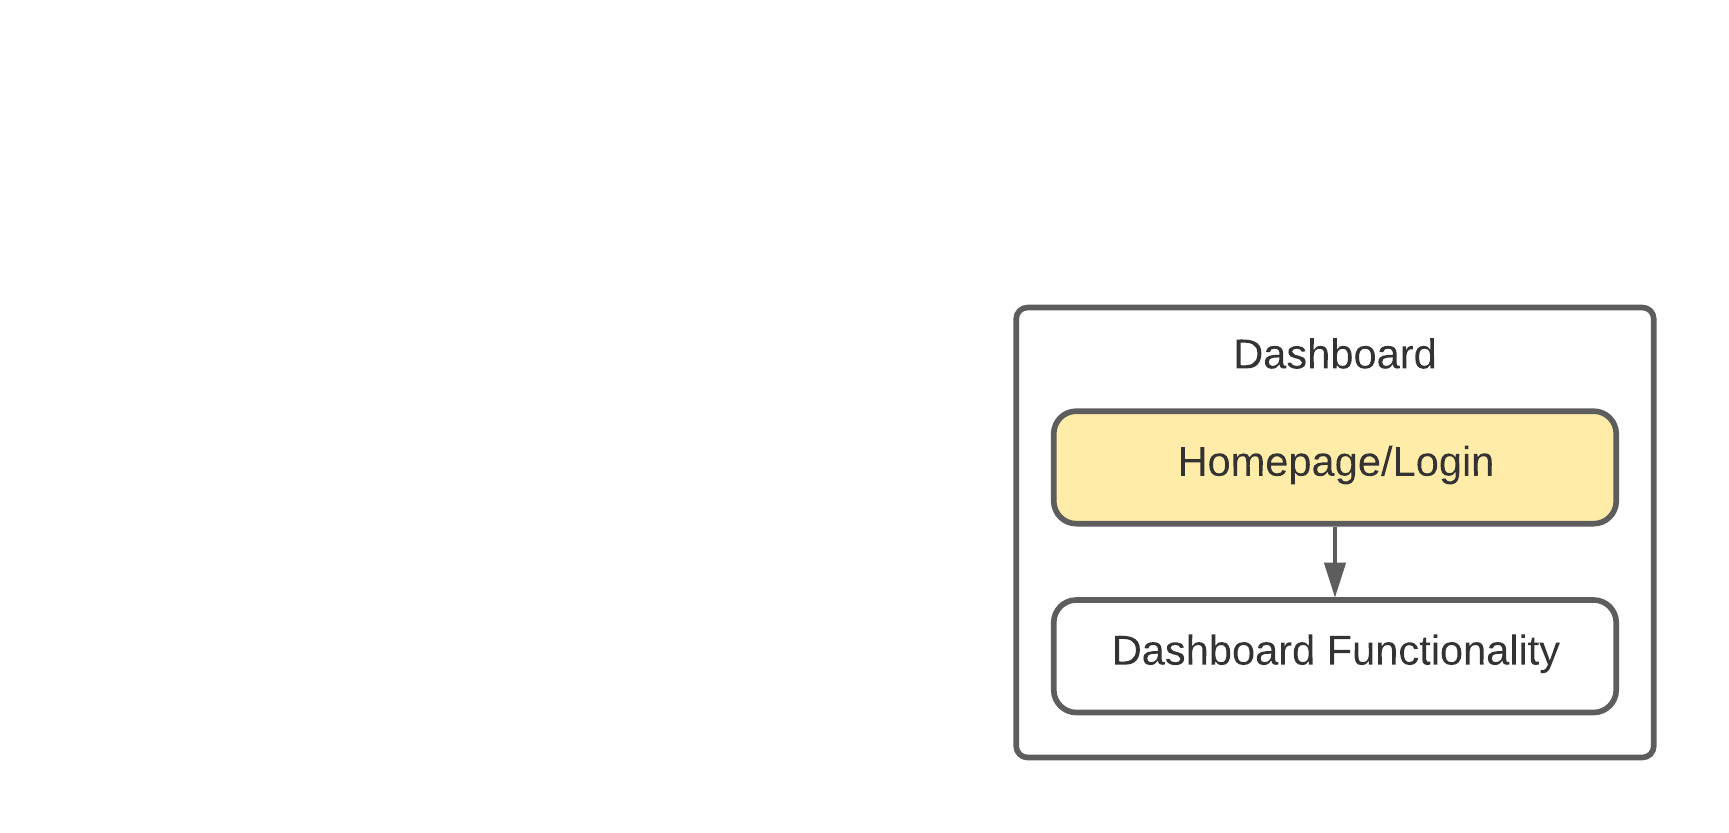
\includegraphics[width=0.60\textwidth]{images/Dashboard_Pic1} % Image
 \caption{Homepage/Login Functionality} % Caption
\end{figure}

\subsubsection{Homepage/Login Hardware}
No Hardware is used.

\subsubsection{Homepage/Login Operating System}
No specific requirement for an Operating System.

\subsubsection{Homepage/Login Software Dependencies}
This is dependent on the Firebase authentication so user can sign up as well as Logging in to their account.

\subsubsection{Homepage/Login Programming Languages}
REACT Typescript and CSS are used.

\subsubsection{Homepage/Login Data Structures}
No specific data structures are used here since the login is based on user input and Firebase takes care of the rest.

\subsubsection{Homepage/Login Data Processing}
Data is not being processed in this section..

\subsection{Dashboard}
Initially this page will look as the homepage, where the user will have the option to create an account or sign in. Once signed in, the page will turn into the page containing a degree flowchart along with a sidebar version of a dashboard which will have the option of signing out for users and include some user information.

%%%%%%%%%%%%%%%%%%%%%%%%%%%%%%%%%%%%%%%%%%%%%%%%%%%%%%%%%%
%  BE SURE TO UPDATE THE IMAGE CAPTION
\begin{figure}[h!]
	\centering
 	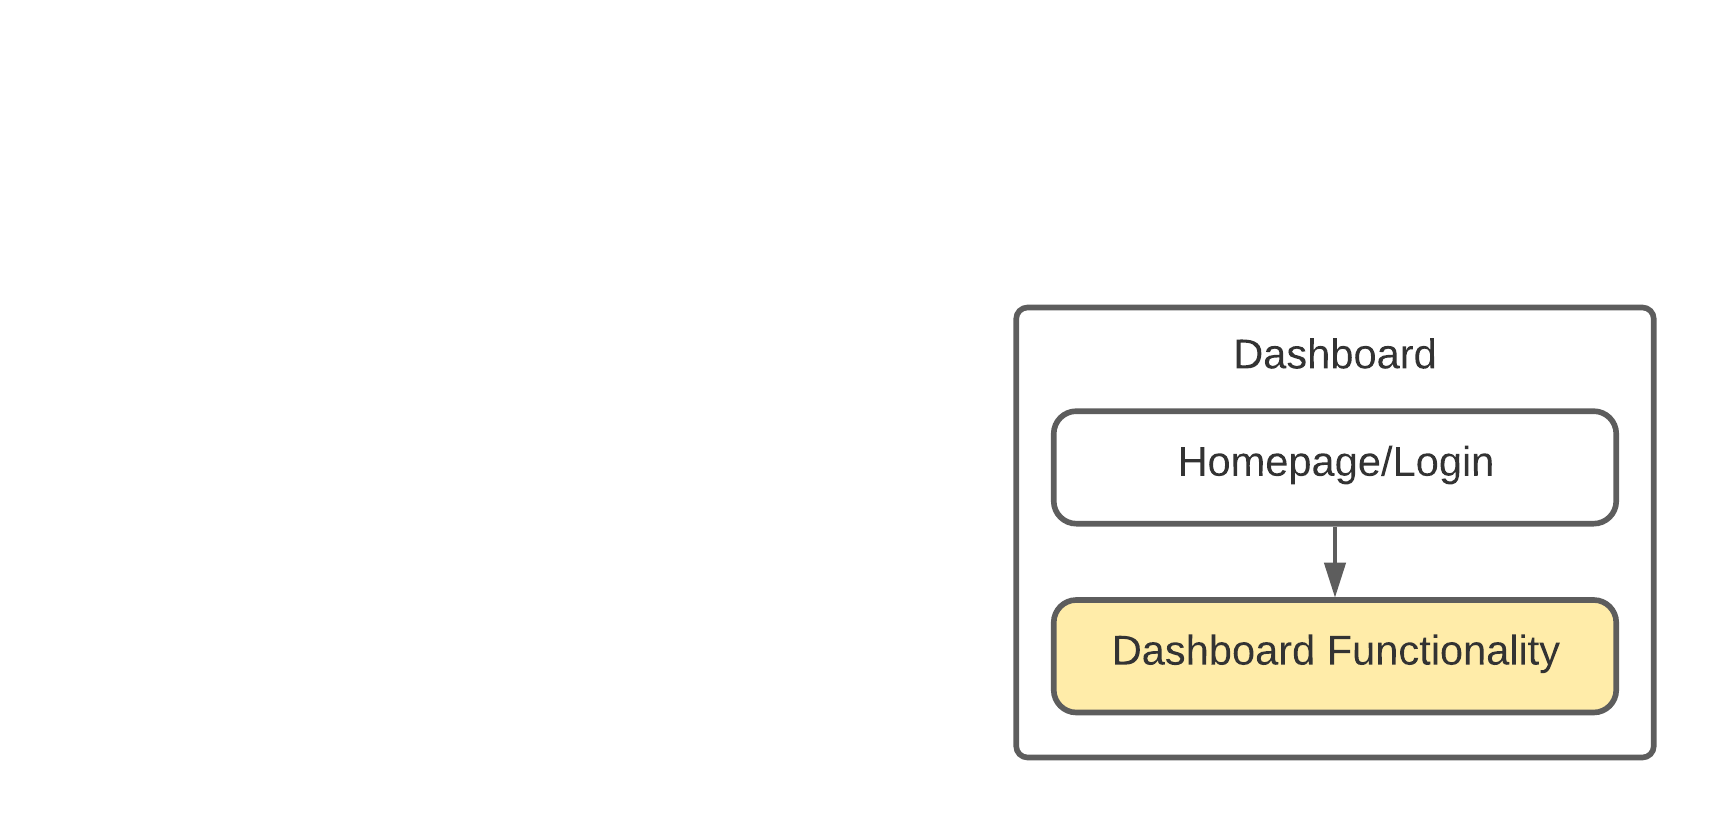
\includegraphics[width=0.60\textwidth]{images/Dashboard_Pic2} % Image
 \caption{Dashboard Functionality} % Caption
\end{figure}

\subsubsection{Dashboard Hardware}
No Hardware is used.

\subsubsection{Dashboard Operating System}
No specific requirement for an Operating System.

\subsubsection{Dashboard Software Dependencies}
This dashboard will have a view flowchart feature where that feature is dependent on a react library called "react-zoom-pan-pinch".

\subsubsection{Dashboard Programming Languages}
REACT Typescript and CSS are used.

\subsubsection{Dashboard Data Structures}
No specific data structures are used here.

\subsubsection{Dashboard Data Processing}
Data is not being processed in this section.


